\chapter{Materials and Methods}

This chapter focus on describing the used materials and methods utilized in this thesis. The acoustic emission tests (Section \ref{sec:AETest}) had 3 separate data acquisition systems, one using an industrial device (DISP-16C) made by Physical Acoustics (PAC), one with another industrial device (AMSY-5) made by Vallen Systems and a custom one denominated Streaming.

Both Streaming and Vallen data were analysed throughout the project duration, however, this thesis concentrates solely on the Streaming data. Both are similar in the way that they acquire temporal data from the AE (not its parameters), however, the AE waveforms captured by the Vallen system had several disadvantages when compared to the Streaming counterpart.

The Vallen data is a collection of fixed length AEs concatenated to form a $L \times N$ matrix where $L$ is the AE length and $N$ the number of captured AEs. This matrix was provided as a MATLAB formatted data file (.MAT) containing the waveform using 64-bit double-precision floating-point format. Unfortunately, this system is not guaranteed to capture all waveforms, this severely hinders some essential preprocessing stages (Sections \ref{sec:TOFDRemoval} and \ref{sec:bombRemoval}), making it a rather unreliable (the captured AE may not be from the crack propagation) and with no means of improving its reliability, therefore all of the Vallen data was discarded.

Thus, this chapter begins detailing the destructive test done, extends to the raw data format used, describes all the preprocessing done and the reasoning behind it, then details the waveform capture procedure all the way to creating the final dataset used to train a neural network model (Section \ref{sec:ann}) with parameters from both the AE temporal data and its frequency spectrum.


\section{Acoustic Emission Test} \label{sec:AETest}

The AE tests were performed by engineers of the Physical Metallurgy Laboratory (LAMEF) at the Federal University of Rio Grande do Sul (UFRGS). It uses a close-ended steel (API XL 60 series) pipe with $20$ inch diameter, $40$ metre length and $1.45$ centimetres of thickness, a semi-elliptical pre-crack extending until half of its thickness (approximately $0.7 cm$) was inserted at half its length.

%mention the rubber cape !!!!!!!!!!

The hydrostatic test consists of a gradual increase of pressure (after filling the tube) followed by plateaus until it bursts (Figure \ref{fig:pressure_time}), this gradual increase is denominated \textit{cycle}. In total, $4$ (four) tests were done, with the first one discarded since it did not burst. They were denominated CP1, CP2, CP3 and CP4 respectively.

\begin{figure}[H]
	\centering
	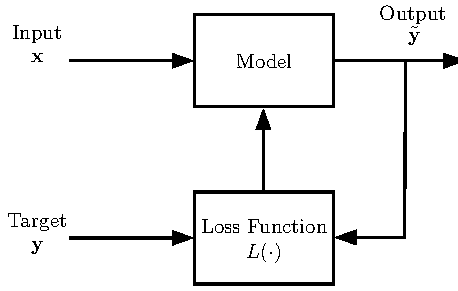
\includegraphics[width=0.1\textwidth]{sup_learning_schematic}
	\caption{Pressure and Crack Dimension for Test CPX}
	\label{fig:pressure_time}
\end{figure}

A sensor array was then disposed on top of the naked steel and the rubber cape (Figure \ref{fig:sensor_disposition}) throughout the tube's length. Immediately surrounding the crack a couple of ultrasound sensors were placed to measure its propagation throughout the test, those work based on Time-of-flight diffraction ultrasonics (TOFD) \cite{charlesworthEngineeringApplicationsUltrasonic2001}, \cite{silkPotentialScatteredDiffracted1975} and are named with respect to the technique (TOFD sensors).

% mention TOFD -> AE sensor or AE sensor -> TOFD ?

\begin{figure}[H]
	\centering
	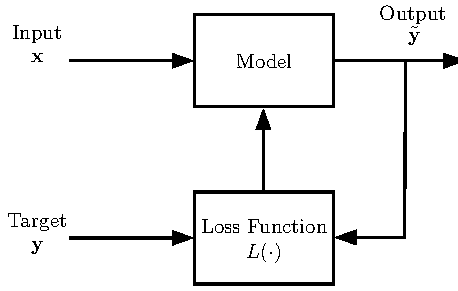
\includegraphics[width=0.1\textwidth]{sup_learning_schematic}
	\caption{Sensor Array Disposition for Test CP3}
	\label{fig:sensor_disposition}
\end{figure}

Three different streaming sensors (Figure \ref{fig:sensor_disposition}) were used, the R1.5 \cite{physicalacousticsR1520KHz}, R15\cite{physicalacousticsR15IAST150KHz} and WD \cite{physicalacousticsWD100900KHz} sensors. Their inner workings and configuration (including conditioning circuits) will not be discussed in this work. It is important to note however, that they work on different frequency ranges (Table \ref{tab:sensor_freq}) and naturally have diverse responses.

\begin{table}[H] \label{tab:sensor_freq}
	\centering
	\caption{Streaming Sensors Frequency Range.}
	\begin{tabular}{cc}
		\hline
		Sensor & Frequency Range (kHz) \\ \hline
		R1.5   & 5 - 20                \\
		R15    & 50 - 400              \\
		WD     & 100 - 900             \\ \hline
	\end{tabular}
\end{table}

These sensors were then sampled using a (not specified) 16 bit Analogue-to-Digital Converter (ADC) at $2.5 GHz$ during the whole test, their data was then put into a special formatted file created by National Instruments (NI), the Technical Data  Management Streaming (TDMS) file \cite{nationalinstrumentsNITDMSFile}. 


\section{Streaming Raw Data}\label{sec:streamingRawData}

Normally, these files can be opened using some specific NI software like \textit{DIAdem} but the LAMEF engineers made slight modifications (Figure \ref{fig:lamef_mods}) when saving the ADC data, using a $32 bit$ word (normally holding one sample) made of two concatenated $16 bit$ integers (that came from the ADC), thus effectively doubling the amount of data stored without requiring additional space.

\begin{figure}[H]
	\centering
	\def\svgwidth{0.7\columnwidth}
	\input{images/low_level_mod_lamef_.pdf_tex}
	\caption{Low-Level Modifications Done to Signal Acquisition.}
	\label{fig:lamef_mods}
\end{figure}


In order to read the TDMS files, LAMEF provided a special compiled LABView routine that transforms each TDMS file to a binary one and a MATLAB script that loads the file to memory. Out of all the tests, only the first one (CP1) did not burst, even after $5$ filling cycles, since identifying the burst is essential (Section \ref{sec:objective}) all CP1 data was discarded and it will not be discussed any further.

A single TDMS file translates to roughly $6.7$ seconds (Figure \ref{fig:tdms_example}), containing $2^{24}$ samples taken from its $16$ different sensors (channels) leading to a $2^{24} \times 16$ integer (16-bit) matrix. In sum (Table \ref{tab:streaming_data}), all data came from (eventually) ruptured ducts and theoretically contain useful data.

\begin{table}[H]\label{tab:streaming_data}
	\centering
	\caption{Hydrostatic Test Summary}
	\resizebox{\columnwidth}{!}{%
	\begin{tabular}{ccccccc}
		\hline
		Test & Date       & \thead{Pre-Crack Depth\\ (millimetres)} & \thead{Rupture Cycle} & \thead{Pressure\\ at Rupture\\ (bar)} & \thead{Data Volume\\ (Gigabytes)}  & Files\\ \hline
		CP1  & 18/03/2015 & 5.5                           & X             & -                         & 3900    & X               \\
		CP2  & 28/07/2015 & 7.9                           & 1             & 230                       & 900     & 1513               \\
		CP3  & 06/11/2015 & 6.6                           & 1             & 264                       & 900 	& 1500                    \\
		CP4  & 23/05/2016 & 7.0                          & 2             & 283                       & 1500	&  4261                \\ \hline
	\end{tabular}%
}
\end{table}

\begin{figure}[H]
	\centering
	\begin{subfigure}{.5\textwidth}
		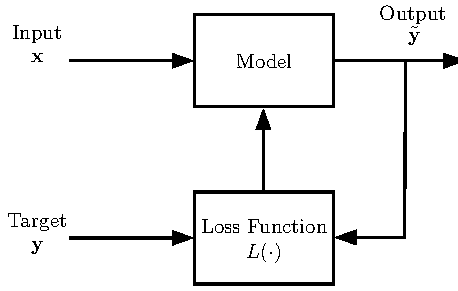
\includegraphics[width=0.1\linewidth]{sup_learning_schematic}
		\caption{TDMS File 900, Channel 12.}
		\label{fig:tdms_example_a}
	\end{subfigure}%
	\begin{subfigure}{.5\textwidth}
		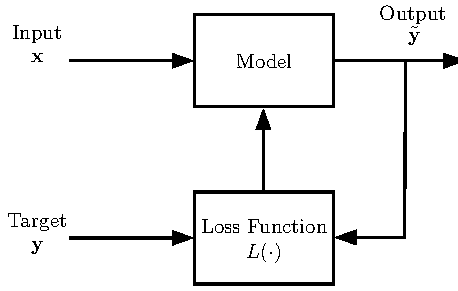
\includegraphics[width=0.1\linewidth]{sup_learning_schematic}
		\caption{TDMS File 900, Channel 7.}
		\label{fig:tdms_example_b}
	\end{subfigure}
	\caption{Data from TDMS File 900, Both Channel 12 (a) and 7 (b) From Test CP3 with Zero (0) Mean.}
	\label{fig:tdms_example}
\end{figure}

\section{Preprocessing} \label{sec:preprocessing}
The preprocessing was likely the lengthiest part of this thesis, it is mainly divided in 3 big blocks, an initial resolution analysis (Section \ref{sec:resAnalysis}) to determine which files contain useful information, a TOFD signal removal (Section \ref{sec:TOFDRemoval}) and a final identification and cleaning of the pressure bomb AE signal (Section \ref{sec:bombRemoval}).

These three stages are invaluable for treating the enormous amount of data ($\approx$ 1TB per test) and coming up with a reliable and efficient way to extract AE from the propagating crack (Section \ref{sec:waveCapture}). 

\subsection{Resolution Analysis}\label{sec:resAnalysis}

Upon first inspection, not all files seemed to contain relevant data (Figure \ref{fig:tdms_example_a}), most of them contained only a noise bar (Figure \ref{fig:tdms_example_b}) thus creating the first problem, determining which files (and channels) contained relevant information so that time would not be wasted trying to find AE waves immersed on noise.

One simple way to determine digital signal quality is through its resolution, signals that are encoded using 10 bits (therefore 1024 digital levels) should have more valuable information than signals encoded with, for instance, 2 bits (therefore 4 digital levels). Using that as a base, it was heuristically stipulated that 8 bits would be the bare minimum (since it gives approximately $1\%$ of the ADC's dynamic range).

The count of digital levels and effective bits used to encode each file and channel was calculated (Figure \ref{fig:res_analysis_example}) and only those that had a minimum of 8 bits were considered good enough to be further inspected.

\begin{figure}[H]
	\centering
	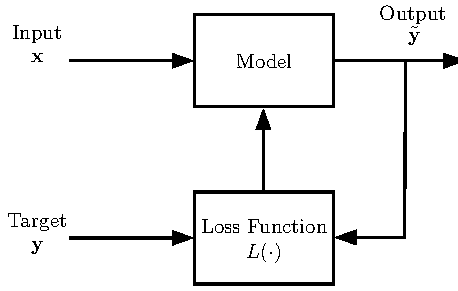
\includegraphics[width=0.1\textwidth]{sup_learning_schematic}
	\caption{Sensor Array Disposition for Test CP3}
	\label{fig:res_analysis_example}
\end{figure}

\subsection{TOFD Removal} \label{sec:TOFDRemoval}

%need to discuss WHY using TOFD and why it must be removed!!!!!

TOFD was not a concern in previous works (Section \ref{sec:biblographyReview}) since it was not evident (even though it can be seen analysing the parameter data). This however, is not true when working with Streaming data, the TOFD signal is clear and has a well defined period and also comes in blocks (Figure \ref{fig:TOFD_example}).

Each block consist of 5 AEs separated by $20 ms$ (Figure \ref{fig:TOFD_example_b}) and each block is $1$ second away from each other (Figure \ref{fig:TOFD_example_a}). These well defined periods can then be used to completely remove all TOFD signals from the entire test.

\begin{figure}[H]
	\centering
	\begin{subfigure}{.5\textwidth}
		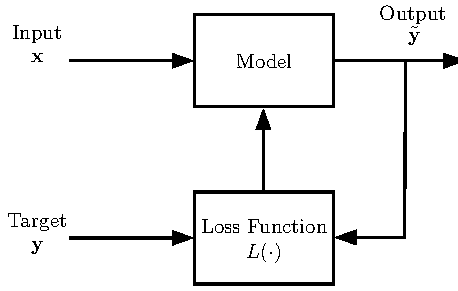
\includegraphics[width=0.1\linewidth]{sup_learning_schematic}
		\caption{TDMS File 900, Channel 12.}
		\label{fig:TOFD_example_a}
	\end{subfigure}%
	\begin{subfigure}{.5\textwidth}
		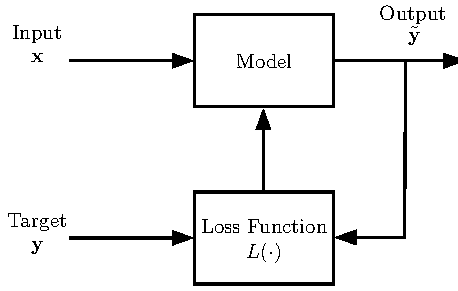
\includegraphics[width=0.1\linewidth]{sup_learning_schematic}
		\caption{TDMS File 900, Channel 12 Focused on a Single TOFD Block}
		\label{fig:TOFD_example_b}
	\end{subfigure}
	\caption{Data from TDMS File 900, Highlighting the TOFD Characteristics.}
	\label{fig:TOFD_example}
\end{figure}

To remove those, it is necessary to first identify it, without going into much detail (those are in Section \ref{sec:waveCapture}) a threshold level is defined for each file/channel combination and each point is compared to that threshold, if its amplitude surpasses it, it receives a 1 (TRUE) and 0 (FALSE) if not (Figure \ref{fig:TOFD_thr_example}).

\begin{figure}[H]
	\centering
	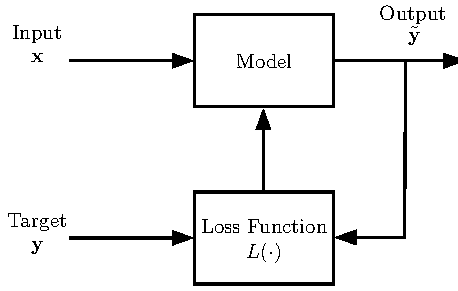
\includegraphics[width=0.1\textwidth]{sup_learning_schematic}
	\caption{Data from TDMS File 900, Channel 12 Containing the Threshold and Indexes that Respectively Surpass It.}
	\label{fig:TOFD_thr_example}
\end{figure}

Once the beginning of each TOFD wave is found, a simple check is done to verify if they are separated by $20 ms +- 10\%$. If so, their indexes are saved and the waves are thus identified. In order to allow a finer control over the TOFD block removal, an additional number of samples is taken from both before and after each wave (Figure \ref{fig:TOFD_window_example}). A total of $50000$ samples ($25000$ for each side) was chosen to guarantee the entire block removal, the downside is that any AE that happens to fall inside a TOFD block is also lost, however, considering that each block takes $100 ms$ each second, that equates to $10\%$ of data being discarded, which is quite acceptable.

\begin{figure}[H]
	\centering
	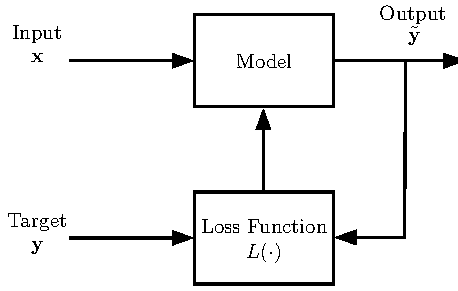
\includegraphics[width=0.1\textwidth]{sup_learning_schematic}
	\caption{Removal of Time-Of-Flight-Diffraction Sensor Signal.}
	\label{fig:TOFD_window_example}
\end{figure}


\subsection{Pressure Bomb Removal} \label{sec:bombRemoval}

Noise from the pressure bomb was also not considered in previous works (Section \ref{sec:bibliographyReview}) and it is an indispensable part of the test, used to fill and pressure the duct. This was discovered by accident when, by analysing multiple files at once, a huge unknown (and somewhat periodic) signal appeared (Figure \ref{fig:pressure_bomb}).

\begin{figure}[H]
 	\centering
 	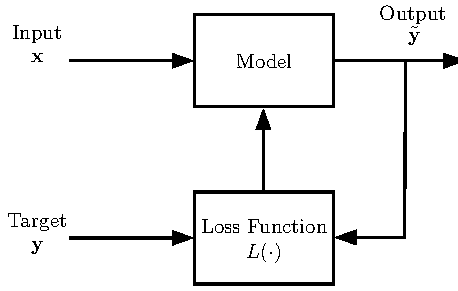
\includegraphics[width=0.1\textwidth]{sup_learning_schematic}
 	\caption{Data From TDMS Files 750-770, Channel 7.}
 	\label{fig:pressure_bomb}
\end{figure}
 
Once crossing the files in which that signal appeared with the logs provided by the LAMEF engineers, it was possible to infer that these signals only appeared at the beginning and end of pressure rising, thus concluding that it is indeed a AE signal generated by the bomb and not the crack propagating.

Its removal was done manually, all $7000$ more files were checked $10$ at a time (a total of more than $700$ different plots) and all files that had even a portion of this signal were discarded.

\section{Wave Capture}\label{sec:waveCapture}

Both Section \ref{sec:preprocessing} and this one contain all that was done in order to transform over $3$ Terabytes of noise filled data into a usable, clean and expandable database containing useful acoustic emission data.

It begins by defining a \textit{noise level} for each file/channel combination and using this information to create a floating threshold level that works similar to that described in Section \ref{sec:TOFDRemoval}, once that threshold is exceed (both positive or negatively) the beginning of a "hit" is defined, and specific timing parameters (Section \ref{sec:timingParameters}) are used to determine its end, thus extracting individual AE waves.

For each of those waves an array of time-domain parameters (Section \ref{sec:AEParameters}) is calculated alongside its power spectrum (Section \ref{sec:frequencyData}). Both are then processed (Section \ref{sec:modelDefinition}) again to be used as input for the neural network.

\subsection{Estimating Noise Level}\label{sec:noiseLevel}

Normally, AE tests use industrial equipment with a fixed Threshold (a level that when exceeded triggers the wave capture) which may or may not be changed throughout the test by its technician. However, instead of trying to define a fixed level for each channel and file, a fluctuating limit was created based on the level of noise for each file/channel. This is interesting since the signal to noise ratio (SNR) can (and does) change a lot because of the varying amplitude of the AE signals (Section \ref{sec:dataDetailing}). Using a volatile limit based on the noise level itself is an attempt to stabilize the SNR for each captured wave.

It is based on a simple metric of standard deviation (Equation \ref{eq:std_def}) applied to each file and channel. In other words, suppose the data from one channel, a $2^{24} \times 1$ array, knowing that AE is a relatively rare event and that there exists a bar of white noise (Figure \ref{fig:tdms_example}), it is safe to say that this array is mostly composed of Gaussian white noise. 

\begin{equation}\label{eq:std_def}
	\sigma_{X} = \sqrt{E[(X-\mu_{X})^{2}]} = \sqrt{\frac{1}{N}\sum_{1}^{N} (x_{i} - \mu_{X})^{2}}
\end{equation}

Where $X$ is the array of size $N=2^{24}$, $\sigma_{X}$ is its standard deviation, $\mu_{X}$ its mean and $x_{i}$ the $i$th array element. Considering that this is composed mostly of Gaussian white noise, it is possible to state:

\begin{equation}
	Noise_{X} \approx 3\sigma_{X}
\end{equation}

This provides a pretty good noise level estimate (Figure \ref{fig:noise_example}) that is then (heuristically) amplified by a factor of $3$ to create a fluctuating threshold able to isolate acoustic emissions.

\begin{figure}[H]
	\centering
	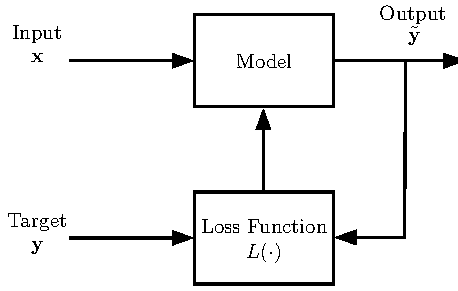
\includegraphics[width=0.1\textwidth]{sup_learning_schematic}
	\caption{Data From TDMS File 900, Channel 7 Highlighting the Noise Level}
	\label{fig:noise_example}
\end{figure}

\subsection{Timing Parameters}\label{sec:timingParameters}

Defining the threshold is but the first step in completely extracting AE information from the data. The DISP16C (used on professional AE tests) user's manual \cite{mistrasgroupDiSPAEwinUSER2011} specifies 3 timing parameters used to capture AE, these are the Hit Definition Time (HDT), Hit Lockout Time (HLT) and Peak Definition Time (PDT). However, PDT is used to determine which peak is the highest (important for calculating AE parameters) while capturing the wave at real time. Since this work uses static data, determining the highest peak makes no sense because there is only one highest peak for each hit (the maximum amplitude), therefore its definition will not be covered in this thesis, if needed, the reader can find it at \cite{mistrasgroupDiSPAEwinUSER2011}.

HDT is the most important parameter and is used to define and fix the end of the "hit". Suppose a signal that exceeds the threshold at a certain time $t_{0}$, once HDT seconds has elapsed while the signal had no threshold crossings (stayed under the threshold) a hit and its end are defined. If one sets this parameter too high, adjacent events may appear as a single hit and if set too low, a single AE may be separated into multiple hits. 

%% SHOW THE HDT IMPORTANCE BY APPLYING IT TO A FEW FIGURES!!! THIS IS GONNA TAKE SOME TIME

HLT can be interpreted as a "dead time" after the definition of a hit, it is a slot of time where no hit can begin even if the signal exceeds the threshold. It is used to eliminate lower amplitude echoes that can occur from the AE's reflection throughout the system. It used to have more importance in the 1980's when computational power was rather limited \cite{mistrasgroupDiSPAEwinUSER2011}.

The tuning of these hyper-parameters is not studied in this thesis since the script made to capture the waves takes around $8$ hours for each CP, so it would be extremely time-consuming and deviate from the main objective of this work, although the author would highly recommend this analysis. Those parameters are then defined as suggested by the LAMEF engineers:

\begin{itemize}
	\item HDT: $1000\mu s$
	\item HLT: $800\mu s$
	\item PDT: N/A 
\end{itemize}

This concludes all necessary steps to extract useful

\subsection{Acoustic Emission Parameters}\label{sec:AEParameters}
\subsection{Frequency Data}\label{sec:frequencyData}

\section{Database Structure}

\section{Model Definition} \label{sec:modelDefinition}

\subsection{Network Size}
\subsection{\textit{Transition Time Estimation}}
\subsection{Relevance Analysis}
\subsection{Relevance Analysis}

